\documentclass[border=4pt]{standalone}
\usepackage{tikz}\usetikzlibrary{arrows.meta,positioning,calc}
\usepackage{amsmath,amssymb}
\begin{document}
\sffamily\small
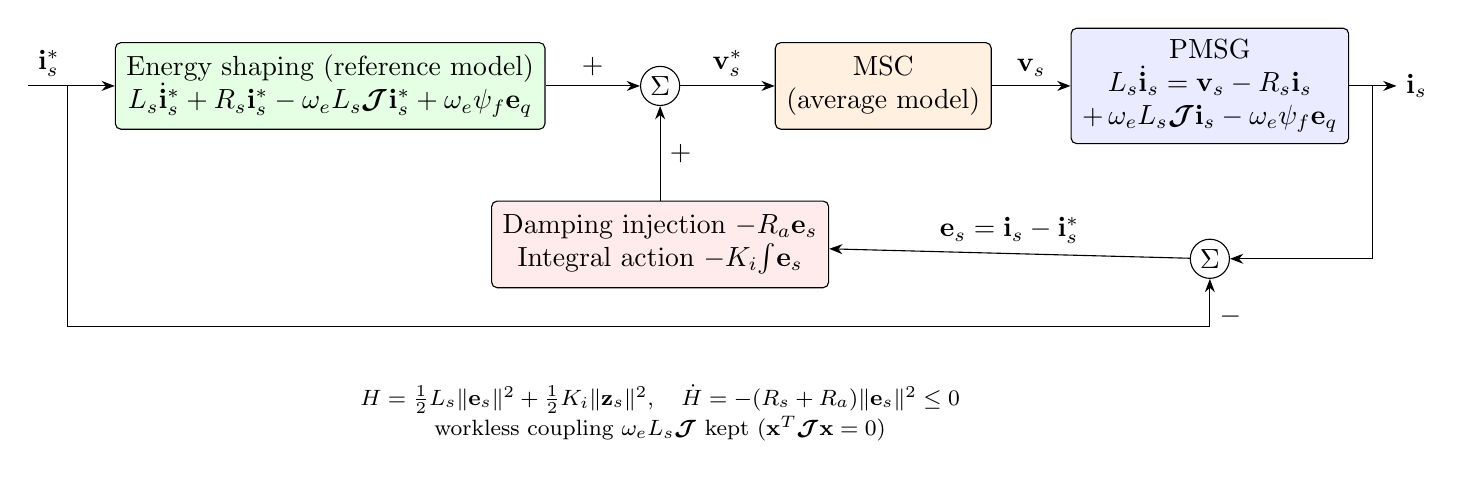
\begin{tikzpicture}[>=Stealth, node distance=7mm and 10mm,
  blk/.style={draw, rounded corners=2pt, minimum height=11mm, align=center, inner sep=4pt, fill=#1},
  sum/.style={draw, circle, inner sep=1.5pt, fill=white}]
\node[blk=green!10] (ff) {Energy shaping (reference model)\\$L_s\dot{\mathbf i}_s^*+R_s\mathbf i_s^*-\omega_eL_s\boldsymbol{\mathcal J}\mathbf i_s^*+\omega_e\psi_f\mathbf e_q$};
\node[sum, right=12mm of ff] (s) {$\Sigma$};
\node[blk=orange!12, right=12mm of s] (conv) {MSC\\(average model)};
\node[blk=blue!8, right=of conv] (pmsg) {PMSG\\$L_s\dot{\mathbf i}_s=\mathbf v_s-R_s\mathbf i_s$\\$+\,\omega_eL_s\boldsymbol{\mathcal J}\mathbf i_s-\omega_e\psi_f\mathbf e_q$};
\node[blk=red!8, below=12mm of s] (damp) {Damping injection $-R_a\mathbf e_s$\\Integral action $-K_i\!\int\!\mathbf e_s$};
\node[sum, below=12mm of pmsg] (e) {$\Sigma$};
\draw[->] ($(ff.west)+(-11mm,0)$) node[above right]{$\mathbf i_s^*$} -- (ff);
\draw[->] (ff) -- node[above]{$+$} (s);
\draw[->] (s) -- node[above]{$\mathbf v_s^*$} (conv);
\draw[->] (conv) -- node[above]{$\mathbf v_s$} (pmsg);
\draw[->] (pmsg.east) -- ++(6mm,0) node[right]{$\mathbf i_s$};
\draw[->] ($(pmsg.east)+(3mm,0)$) |- (e);
\draw[->] ($(ff.west)+(-6mm,0)$) |- ($(e.south)+(0,-6mm)$) -- node[right, pos=0.2]{$-$} (e.south);
\draw[->] (e) -- node[above]{$\mathbf e_s=\mathbf i_s-\mathbf i_s^*$} (damp);
\draw[->] (damp) -- node[right]{$+$} (s);
\node[below=11mm of damp, align=center, font=\footnotesize] {$H=\frac12L_s\|\mathbf e_s\|^2+\frac12K_i\|\mathbf z_s\|^2,\quad \dot H=-(R_s+R_a)\|\mathbf e_s\|^2\le0$\\ workless coupling $\omega_eL_s\boldsymbol{\mathcal J}$ kept ($\mathbf x^T\boldsymbol{\mathcal J}\mathbf x=0$)};
\end{tikzpicture}
\end{document}
